% \documentclass[11pt,twoside]{book} %纸质版用twoside
\documentclass[12pt,oneside]{book} %电子版用oneside
\usepackage{setspace}

% \documentclass{article}

%%%%%%%%%%%%%%%%%%%%%%%%%%%%%%%%%%%%%%%%%%%%%%%%%%
%%%%%%%%%%%%%%%%%%%%% preamble %%%%%%%%%%%%%%%%%%%
%%%%%%%%%%%%%%%%%%%%%%%%%%%%%%%%%%%%%%%%%%%%%%%%%%

\usepackage[mono=false]{libertine} % new linux font, ignore mono

\usepackage{luatex85}

%\renewcommand{\baselinestretch}{1.05}
\usepackage{amsmath,amsthm,amssymb,mathrsfs,amsfonts,dsfont}
\usepackage{epsfig,graphicx}
\usepackage{tabularx}
\usepackage{blkarray}
\usepackage{slashed}
\usepackage{color}
\usepackage{listings}
\usepackage{caption}
% \usepackage{fullpage}
\usepackage{lipsum} % provides dummy text for testing
\usepackage[toc,title,titletoc,header]{appendix}
\usepackage{minitoc}
\usepackage{color}
\usepackage{multicol} % two-col ToC
\usepackage{bm}
\usepackage{imakeidx} % before hyperref
\usepackage{hyperref}
\usepackage{indentfirst}
\setlength{\parindent}{2em}


% link colors settings
\hypersetup{
    colorlinks=true,
    citecolor=magenta,
    linkcolor=blue,
    filecolor=green,      
    urlcolor=cyan,
    % hypertexnames=false,
}
\usepackage[capitalise]{cleveref}
\usepackage{subcaption}
\usepackage{enumitem}
\usepackage{mathtools}
\usepackage{physics}
\usepackage[linesnumbered,ruled,vlined,algosection]{algorithm2e}
\SetCommentSty{textsf}
\usepackage{epigraph}
\epigraphwidth=1.0\linewidth
\epigraphrule=0pt

% adjust margin
\usepackage[margin=2.3cm]{geometry}
\headheight13.6pt


\usepackage{graphicx}
\usepackage[justification=centering]{caption} % 图注居中
\usepackage{setspace}
\usepackage{geometry}
\usepackage{float}
\usepackage{hyperref}
\usepackage[utf8]{inputenc}
\usepackage[english]{babel}
\usepackage{framed}


\newcommand{\HRule}[1]{\rule{\linewidth}{#1}}





\setstretch{1.2}
% \geometry{
%     textheight=9in,
%     textwidth=5.5in,
%     top=1in,
%     headheight=12pt,
%     headsep=25pt,
%     footskip=30pt
% }





%%%%%%%%%%%%%%%% thmtools %%%%%%%%%%%%%%%%%%%%%

\usepackage{thmtools}
\usepackage[dvipsnames]{xcolor}
\usepackage[most]{tcolorbox}
\usepackage{enumerate}

\colorlet{LightGreen}{Green!15} %def
\colorlet{LightBlue}{Blue!15} %thm
\colorlet{LightOrange}{Orange!15} %lem
\colorlet{LightGray}{Gray!15}  %prop
\colorlet{LightRed}{Red!40} %cor
\colorlet{LightYellow}{Yellow!15} %exa


% \newtcbtheorem[
%   number within = chapter % 按每个 chapter 分别编号
% ]{definition% 环境名
% }{Definition% 这个参数可以设成“定理”“引理”“推论”等,编号就会变成“定理 1.1”“引理 1.1”“推论 1.1”等
% }{
%   attach title to upper = \par\vspace{1ex}, % 不要单独的标题栏,定理名完了之后分段,加上适量空白
%   separator sign = \quad, % 定理编号和定理名字之间用什么分隔;默认是冒号
%   sharp corners, % 直角;默认是圆角
%   enhanced jigsaw, frame hidden, % 隐藏 tcb 边框
%   colback = LightGreen, % 背景色
%   coltitle = blue!20!cyan!80!black, % 标题(定理编号和名字)的颜色
%   fonttitle = \sffamily\small, % 标题(定理编号和名字)的字体
%   description font = \normalsize, % 定理名字的字体
%   fontupper = \normalfont, % box 内的字体
% }{def% label 前缀
% }

\newtcbtheorem[
  number within = chapter % 按每个 chapter 分别编号
]{definition% 环境名
}{Definition% 这个参数可以设成“定理”“引理”“推论”等,编号就会变成“定理 1.1”“引理 1.1”“推论 1.1”等
}{
  sharp corners, % 直角;默认是圆角
  colback=Green!5,
  colframe=Green!50!black,
  fonttitle=\sffamily\small
}{def% label 前缀
}


\newtcbtheorem[
  number within = chapter % 按每个 chapter 分别编号
]{theorem% 环境名
}{Theorem% 这个参数可以设成“定理”“引理”“推论”等,编号就会变成“定理 1.1”“引理 1.1”“推论 1.1”等
}{
  sharp corners, % 直角;默认是圆角
  colback=yellow!10,
  colframe=yellow!50!black,
  fonttitle=\sffamily\small
}{thm% label 前缀
}


\newtcbtheorem[
  number within = chapter % 按每个 chapter 分别编号
]{proposition% 环境名
}{Proposition% 这个参数可以设成“定理”“引理”“推论”等,编号就会变成“定理 1.1”“引理 1.1”“推论 1.1”等
}{
  sharp corners, % 直角;默认是圆角
  colback=Red!5,
  colframe=Red!50!black,
  fonttitle=\sffamily\small
}{prop% label 前缀
}

\newtcbtheorem[
  number within = chapter % 按每个 chapter 分别编号
]{corollary% 环境名
}{Corollary% 这个参数可以设成“定理”“引理”“推论”等,编号就会变成“定理 1.1”“引理 1.1”“推论 1.1”等
}{
  sharp corners, % 直角;默认是圆角
  colback=Blue!5,
  colframe=Blue!50!black,
  fonttitle=\sffamily\small
}{cor% label 前缀
}

\newtcbtheorem[
  number within = chapter % 按每个 chapter 分别编号
]{lemma% 环境名
}{Lemma% 这个参数可以设成“定理”“引理”“推论”等,编号就会变成“定理 1.1”“引理 1.1”“推论 1.1”等
}{
  sharp corners, % 直角;默认是圆角
  colback=Gray!10,
  colframe=Gray!50!black,
  fonttitle=\sffamily\small
}{lem% label 前缀
}


\newtcbtheorem[
  number within = chapter % 按每个 chapter 分别编号
]{example}
{Example}%
  {
    enhanced, breakable,
    colback = white, colframe = purple, colbacktitle = purple,
    attach boxed title to top left = {yshift = -2mm, xshift = 5mm},
    boxed title style = {sharp corners},
    fonttitle=\sffamily\small
  }
{exa}


\newtcbtheorem[
  number within = chapter % 按每个 chapter 分别编号
]{exercise}
{Exercise}%
  {
    enhanced, breakable,
    colback = white, colframe = cyan, colbacktitle = cyan,
    attach boxed title to top left = {yshift = -2mm, xshift = 5mm},
    boxed title style = {sharp corners},
    fonttitle=\sffamily\small
  }
{exer}


% \declaretheorem[numberwithin=chapter,shaded={rulecolor=LightGreen,
% rulewidth=2pt,bgcolor=LightGreen,
% textwidth=12em}]{definition}

\usepackage{changepage}
\newenvironment{remark}{\underline{\textbf{Remark.}}}{\par}

\newenvironment{proofsolution}
    {\renewcommand\qedsymbol{$\square$}\color{blue}\begin{adjustwidth}{0em}{2em}\begin{proof}[\textit Proof.~]}
    {\end{proof}\end{adjustwidth}}


%%%%%%%%%%%%%%%% index %%%%%%%%%%%%%%%%%%%%%
\begin{filecontents}{index.ist}
% https://tex.stackexchange.com/questions/65247/index-with-an-initial-letter-of-the-group
headings_flag 1
heading_prefix "{\\centering\\large \\textbf{"
heading_suffix "}}\\nopagebreak\n"
delim_0 "\\nobreak\\dotfill"
\end{filecontents}
\newcommand{\myindex}[1]{\index{#1} \emph{#1}}
\makeindex[columns=3, intoc, title=Alphabetical Index, options= -s index.ist]
%%%%%%%%%%%%%%%% index %%%%%%%%%%%%%%%%%%%%%

%%%%%%%%%%%%%%%% ToC %%%%%%%%%%%%%%%%%%%%%
% Link Chapter title to ToC: https://tex.stackexchange.com/questions/32495/linking-the-section-text-to-the-toc
\usepackage[explicit]{titlesec}
\titleformat{\chapter}[display]
  {\normalfont\huge\bfseries}{\chaptertitlename\ {\thechapter}}{20pt}{\hyperlink{chap-\thechapter}{\Huge#1}
\addtocontents{toc}{\protect\hypertarget{chap-\thechapter}{}}}
\titleformat{name=\chapter,numberless}
  {\normalfont\huge\bfseries}{}{-20pt}{\Huge#1}

%%%%%%%%%%%%%%%%%%% fancyhdr %%%%%%%%%%%%%%%%%
\usepackage{fancyhdr}
\pagestyle{fancy} % enable fancy page style
\renewcommand{\headrulewidth}{0.0pt} % comment if you want the rule
\fancyhf{} % clear header and footer
\fancyhead[lo,le]{\leftmark}
\fancyhead[re,ro]{\rightmark}
\fancyfoot[CE,CO]{\hyperref[toc-contents]{\thepage}}

% https://tex.stackexchange.com/questions/550520/making-each-page-number-link-back-to-beginning-of-chapter-or-section
\makeatletter
\def\chaptermark#1{\markboth{\protect\hyper@linkstart{link}{\@currentHref}{Chapter \thechapter ~ #1}\protect\hyper@linkend}{}}
\def\sectionmark#1{\markright{\protect\hyper@linkstart{link}{\@currentHref}{\thesection ~ #1}\protect\hyper@linkend}}
\makeatother
%%%%%%%%%%%%%%%%%%% fancyhdr %%%%%%%%%%%%%%%%%


%%%%%%%%%%%%%%%%%%% biblatex %%%%%%%%%%%%%%%%%
\usepackage[doi=false,url=false,isbn=false,style=alphabetic,backend=biber,backref=true]{biblatex}
\addbibresource{bib.bib}

\newbibmacro{string+doiurlisbn}[1]{%
  \iffieldundef{doi}{%
    \iffieldundef{url}{%
      \iffieldundef{isbn}{%
        \iffieldundef{issn}{%
          #1%
        }{%
          \href{http://books.google.com/books?vid=ISSN\thefield{issn}}{#1}%
        }%
      }{%
        \href{http://books.google.com/books?vid=ISBN\thefield{isbn}}{#1}%
      }%
    }{%
      \href{\thefield{url}}{#1}%
    }%
  }{%
    \href{http://dx.doi.org/\thefield{doi}}{#1}%
  }%
}

% https://tex.stackexchange.com/questions/94089/remove-quotes-from-inbook-reference-title-with-biblatex
\DeclareFieldFormat[article,incollection,inproceedings,book,misc]{title}{\usebibmacro{string+doiurlisbn}{\mkbibemph{#1}}}
% https://tex.stackexchange.com/questions/454672/biblatex-journal-name-non-italic
\DeclareFieldFormat{journaltitle}{#1\isdot}
\DeclareFieldFormat{booktitle}{#1\isdot}
% https://tex.stackexchange.com/questions/10682/suppress-in-biblatex
\renewbibmacro{in:}{}
% add video field: https://tex.stackexchange.com/questions/111846/biblatex-2-custom-fields-only-one-is-working
\DeclareSourcemap{
    \maps[datatype=bibtex]{
      \map{
        \step[fieldsource=video]
        \step[fieldset=usera,origfieldval]
    }
  }
}
\DeclareFieldFormat{usera}{\href{#1}{\textsc{Online video}}}
\AtEveryBibitem{
    \csappto{blx@bbx@\thefield{entrytype}}{% put at end of entry
        \iffieldundef{usera}{}{\space \printfield{usera}}
    }
}


%%%%%%%%%%%%%%%%%%%%%%%notations%%%%%%%%%%%%%%%%%%%%%%%%%%%%%%
\newcommand{\F}{\ensuremath{\mathbb{F}}}
\newcommand{\C}{\ensuremath{\mathbb{C}}} 
\newcommand{\R}{\ensuremath{\mathbb{R}}}
\newcommand{\J}{\ensuremath{\mathbb{J}}}
\newcommand{\Q}{\ensuremath{\mathbb{Q}}}
\newcommand{\Z}{\ensuremath{\mathbb{Z}}}
\newcommand{\N}{\ensuremath{\mathbb{N}}}
\newcommand{\K}{\ensuremath{\mathbb{K}}}
\newcommand{\Zo}{\ensuremath{\mathbb{Z}_{\geqslant 0}}} % 非负整数集
\newcommand{\Zi}{\ensuremath{\mathbb{Z}_{\geqslant 1}}} % 正整数集
\newcommand{\id}{\mathrm{id}}
\newcommand{\im}{\mathrm{im}\,}                         % 映射的像
\newcommand{\leqs}{\leqslant}
\newcommand{\geqs}{\geqslant}
\newcommand{\ci}{\mathrm{i}}
\newcommand{\hH}{\mathcal{H}}
\newcommand{\hK}{\mathcal{K}}
\newcommand{\inner}[2]{\langle#1,#2\rangle}

%%%%%%%%%%%%%%%%%%% biblatex %%%%%%%%%%%%%%%%%

%%%%%%%%%%%%%%%%%%%%% glossaries %%%%%%%%%%%%%%%%%
% !TEX root = ./notes_template.tex
% \usepackage[style=super]{glossaries}
% https://www.overleaf.com/learn/latex/Glossaries
\usepackage[style=super,toc,acronym]{glossaries}
\setlength{\glsdescwidth}{1\linewidth}
\makeglossaries

\renewcommand\glossaryname{List of Abbreviations and Symbols}

\newglossaryentry{Q2}{name={$Q_2(f)$},
%sort=Q2,
description={Two-side (bounded) error quantum query complexity}}

\newglossaryentry{real_number}{name={$\mathbb{R}$},description={Real number}}

% \newglossaryentry{gcd}{name={gcd},description={greatest common divisor}}

\newacronym{gcd}{GCD}{Greatest Common Divisor}


\newglossaryentry{svm}{name={SVM},description={Support Vector Machine}}

\newglossaryentry{gd}{name={GD},description={Gradient Descent}}

\newglossaryentry{qft}{name={QFT},description={Quantum Field Theory}}

\newglossaryentry{qm}{name={QM},description={Quantum Mechanics}}

\newglossaryentry{v}{name={$\vec{v}$},description={a vector}}

% physics
\newglossaryentry{hamiltonian}{name={$\hat{H}$},description={Hamiltonian}}

\newglossaryentry{lagrangian}{name={$L$},description={Lagrangian}}
%%%%%%%%%%%%%%%%%%%%% glossaries %%%%%%%%%%%%%%%%%

%%%%%%%%%%%%%%%%%%%%% glossaries-extra %%%%%%%%%%%%%%%%%
% \usepackage[record,abbreviations,symbols,stylemods={list,tree,mcols}]{glossaries-extra}
%%%%%%%%%%%%%%%%%%%%% glossaries-extra %%%%%%%%%%%%%%%%%


% !TEX root = ./notes_template.tex

%%%%%%%%%%%%%%%%%%%%%%%%%%%%%%%%%%%%
%%%%%%%%%%%%%%%%%%%%%%%%%%%%%%%%%%%%
% math
\let\iff\relax
\newcommand{\iff}{\text{ iff }}
\newcommand{\OPT}{\textup{OPT}}

% physics
\newcommand{\acreation}{a^\dagger}



%%%%%%%%%%%%%%%%%%%%%%%%%%%%%%%%%%%%%%%%%%%%%%%%%%
%%%%%%%%%%%%%%%% begin of document %%%%%%%%%%%%%%%
%%%%%%%%%%%%%%%%%%%%%%%%%%%%%%%%%%%%%%%%%%%%%%%%%%

\begin{document}

\title{\bf \huge Study Notes of Numerical Optimization}
\author{Pei Zhong}
\date{Update on \today}

\maketitle

% \newpage
% \let\cleardoublepag\clearpage

\tableofcontents

\begin{spacing}{1}

%%%%%%%%%%%%%%update progress%%%%%%%%%%
\chapter*{Update progress}
\begin{itemize}
    \item {writing ch\ref{chp:Convex Optimization}... \hfill 2023.10.20}
\end{itemize}


%%%%%%%%%%%%%%update progress end%%%%%%%%




%%%%%%%%%%%%%%%preface%%%%%%%%%%%%%
% !TEX root = ../notes_template.tex
\chapter*{Preface}


Notes mainly refer to the following resources:
Convex optimization & duality:
\begin{itemize}
    \item \href{https://web.stanford.edu/~boyd/cvxbook/}{Convex Optimizaiton. Stephen Boyd, Lieven Vandenberghe}
    \item \href{https://link.springer.com/book/10.1007/978-0-387-40065-5}{Numerical Optimization(2nd). Jorge Nocedal, Stephen J.Wright} 
    \item \href{https://cdn.syscop.de/publications/Diehl2016.pdf}{lecture notes from University of Freiburg}
    \item \href{https://faculty.ucmerced.edu/mcarreira-perpinan/teaching/EECS260/lecture-notes.pdf}{lecture notes from University of California}
    \item \href{https://www.uio.no/studier/emner/matnat/math/nedlagte-emner/MAT-INF2360/v13/matinf2360part3.pdf}{Lecture notes for the course MAT-INF2360}
    \item \href{https://www.numerical.rl.ac.uk/people/nimg/msc/lectures/paper.pdf}{An introduction to algorithms for nonlinear optimization} 
    \item \href{https://www.princeton.edu/~aaa/Public/Teaching/ORF523/S16/}{ORF 523 Convex and Conic Optimization}
    \item \href{}{lecture notes from School of Electrical Engineering at Korea Advanced Institute of Science and Technology}
    \item \href{https://www.stat.cmu.edu/~ryantibs/convexopt-F18/}{Convex Optimization: Fall 2018}
\end{itemize}


application:

\begin{itemize}
    \item \href{https://web.eecs.umich.edu/~fessler/course/598/}{Optimization methods for signal and image processing and machine learning}
\end{itemize}



% \par

all the codes in the notes are completed by python. You can get the codes in the following website:
\begin{itemize}
    \item -
\end{itemize}

\par
% In Part I, we will study the basic concepts and several
% mathematical definitions required to understand what convex optimization is as well as how to
% translate an interested problem into a convex problem. We will then explore five instances of
% convex optimization problems: LP, least-squares, QP, SOCP and SDP. Specifically we will focus
% on techniques which serve recognizing (and translating to) such problems. We will also study
% some prominent algorithms for solving such problems. 
% \par
% In Part II, we will study one of the key
% theories in the optimization field, called duality. There are two types of dualities: (1) strong
% duality; (2) weak duality. It turns out that the strong duality is quite useful for gaining some
% algorithmic insights for convex problems. 
% The weal duality helps dealing with difficult non-convex problems, by providing an approximated solution.
% \par 
% In part III, our focus is on continuous optimization (rather than discrete optimization) with special emphasis on nonlinear programming.
% We will Utilize the knowledge of PartI and PartII to mine the optimal solution conditions and 
% solving methods for nonlinear optimization problems. 







\chapter{Preliminary Knowledge}

The goal of this chapter is to refresh your memory on some
topics in linear algebra and multivariable calculus that will be
relevant to the following content. You can use this as a reference
throughout the semester. 

\section{Inner Products and Norms}
\subsection{Inner Products}
Without hypotheses, we use $x\in \R^n$ to denote vectors of $\R^n$ with $x=(x_1,x_2,\cdots,x_n)$ and $x\geqs y$ to denote point-wise order $x_i\geqs y_i,1\leqs i \leqs n$. Then, $\R^n_+$ and $\R^n_{++}$ are defined by $\R^n_+:=\{x\in \R^n\mid x\geqs 0\}$ and  $\R^n_+:=\{x\in \R^n\mid x> 0\}$. Besides, $e_i$ is the $i$-th 
standard basis $e_i=(0,\cdot,0,\mathop{1}\limits^{i},0,\cdots,0)^T$.
\begin{definition}{Inner product and vector norm}{Inner product}
    (i) For given vectors $x,y\in \R^n$, their \textbf{inner product} and the induce \textbf{Euclidean norm}(or, \textbf{$l^2$-norm}) are defined by
    \begin{align*}
        \inner{x}{y} &:=x^Ty = \sum_{i=1}^nx_iy_i\\
        \norm{x}_2 &:=(\inner{x}{x})^{\frac{1}{2}} = \left(\sum\limits_{i=1}^nx_i^2\right)^{\frac{1}{2}}. 
    \end{align*}

    (ii) For a given vector $x\in \R^n$, the \textbf{$l^1$-norm} and \textbf{$l^{\infty}$-norm} are defined by
    \begin{align*}
        \norm{x}_1=\sum_{i=1}^n|x_i|,\norm{x}_{\infty}=\max_{1\leqs i \leqs n}|x_i|.
    \end{align*}
\end{definition}
\begin{proposition}{Fundamental properties of norm}{}
    For $l^p$-norm $\norm{\cdot}_p,p=1,2,\infty$ of the vectors $x,y\in \R^n$, one have

    (i) Positive defininteness: $\norm{x}_p\geqs 0$ and $\norm{x}_p=0\Leftrightarrow x = 0$.

    (ii) Positive Homogeneity: $\norm{kx}_p = k\norm{x}_p$ for $k\geqs 0$.

    (iii) Subadditivity: $\norm{x+y}_p\leqs \norm{x}_p + \norm{y}_p$.
\end{proposition}
\begin{remark}
    Essentially, any functional $p:\R^n\to \R_+$ satisfying the above three properties is a norm of $\R^n$.
\end{remark}

The following inequality plays a important role in theoretical analysis.
\begin{theorem}{Cauchy-Schwarz Inequality}{}
    \begin{equation*}
        \inner{x}{y}=x^Ty\leqs \norm{x}_2\norm{y}_2, x,y\in \R^n,
    \end{equation*}
    the equality holds if and only if $x = ky,k\in \R$ i.e. $x,y$ are parallel.
\end{theorem}

\subsection{Vector Norms}

\subsection{Matrix Norms}
Analogous to vector norm, we could define norm for matrices, here are some frequently used matrix norms:
\begin{definition}{matrix norms}{}
    For a given matrix $A\in \R^{n\times n},$ there are some norms as following:

    (i) \textbf{Frobenius norm}: $\norm{A}_F:=\left(\sum\limits_{i=1}^n\sum\limits_{j=1}^na_{ij}^2\right)^{\frac{1}{2}}$.

  (ii) \textbf{$2$-norm}, or \textbf{spectral norm}: $\norm{A}_2:=\max\limits_{\norm{x}_2=1}\norm{Ax}_2$.
\end{definition}

\begin{definition}{condition number}{}
    For a given matrix $A\in \R^{n\times n}$, the condition of $A$ is defined as
    \begin{align*}
        \kappa(A) = ||A||_2\cdot ||A^{-1}||_2,
    \end{align*}
    If $A$ is singular then $\kappa(A)=\infty$. 
    In numerical analysis the condition number of a matrix $A$ is is a way of describing how well or badly the system
    $Ax=b$ could be approximated. If $\kappa(A)$ is small the problem is well-conditioned and if
    $\kappa(A)$ is large the problem is rather ill-conditioned.
\end{definition}
\begin{remark}
    If $A$ is a symmetric matrix, another expression for the condition number is $\kappa(A) = |\frac{\lambda_{max}}{\lambda_{min}}|$, where $\lambda_{max}$ and $\lambda_{min}$
    denote the largest and smallest eigenvalues of $A$.
\end{remark}

\begin{theorem}{Spectral norm characterization}{equivalent characterization of 2-norm of matrix}
    For a given matrix $A\in \R^{n\times n}$,
    \begin{equation*}
        \norm{A}_2=\max_{\norm{x}=1}\norm{Ax}_2=\left(\lambda_{\max}(A^TA)\right)^{\frac{1}{2}},
    \end{equation*}
    in which $\lambda_{\max}(A)$ is the maximal eigenvalues of $A$. Furthermore, by notation $\lambda(A)$ denoted the set of all eigenvalues of $A$, we have $\norm{A}_2=\max(|\lambda(A)|)$ when $A$ is symmetric.
\end{theorem}
\begin{proof}
    By Cauchy-Schwarz inequality one have
    \begin{equation*}
        \norm{Ax}_2^2=\inner{Ax}{Ax}=x^T(A^TAx)\leqs \norm{x}_2\norm{A^TAx}_2=\norm{A^TAx}_2,\forall \ x\in \R^n,\norm{x}=1,
    \end{equation*}
    and the equality holds if and only if $x,A^TAx$ are parallel, that is $A^TAx =\lambda x$ for some $\lambda\in \R$ i.e. $x$ is an eigenvector of $A^TA$ associated with eigenvalue $\lambda$. Hence
    \begin{equation*}
        \max_{\norm{x}_2=1}\norm{Ax}_2\leqs \max_{\norm{x}_2=1}\left(\norm{x}_2\norm{A^TAx}_2\right)^{\frac{1}{2}}\leqs \max_{\norm{x}_2=1}\left(\norm{x}_2(\lambda\norm{x}_2)\right)^{\frac{1}{2}}\leqs (\lambda_{\max}(A^TA))^{\frac{1}{2}},
    \end{equation*}
    and there is eigenvector $x^*$ associated with maximal eigenvalue $\lambda_{\max}$ of $A^TA$ such that $\norm{Ax^*}_2=(\lambda_{\max}(A^TA))^{\frac{1}{2}}$, therefore $\max\limits_{\norm{x}_2=1}\norm{Ax}_2=(\lambda_{\max}(A^TA))^{\frac{1}{2}}$.

    When $A$ is symmetric, $\lambda_{\max}(A^TA)=\lambda_{\max}(A^2)=(\max(|\lambda(A)|))^2$, then the conclusion is obvious.
\end{proof}

The next property of $2$-norm is common in theoretical analysis. Its proof is similar to theorem \ref{thm:equivalent characterization of 2-norm of matrix} hence it is remained to an exercise.

\begin{corollary}{Compatibility of $2$-norm}{}
For a given $A\in \R^{n\times n},x\in \R^n$,

(i) $\norm{Ax}_2\leqs \norm{A}_2\norm{x}_2$.

(ii) When $A$ is symmetric, the quadratic form has the attained upper bound and lower bound
\begin{equation}
    \lambda_{\min}(A)\norm{x}_2\leqs x^TAx\leqs \lambda_{\max}(A)\norm{x}_2.
\end{equation}

(iii) As a corollary of (ii), $A$ is positive (semi-)definited if and only if $\lambda_{\min}(A)>0(\geqs 0)$.
\end{corollary}


\section{Quadratic Form}

The theoretical analysis and algorithm design always involve matrix, especially symmetric positive definited matrix. We briefly introduction the concept of quadratic form.
\begin{definition}{Quadratic form}{}
    Give a multivariate quadratic function $f:\R^n\to \R,$
    \begin{equation*}
        f(x_1,x_2,\cdots,x_n) = a_{11}x_1^2+\cdots+a_{nn}x^2_n+2a_{12}x_1x_2+\cdots + 2a_{n-1,n}x_{n-1}x_n =\sum_{i=1}^n\sum_{j=1}^na_{ij}x_ix_j,
    \end{equation*}
    one rewrite $f$ as 
    \begin{equation*}
        f(x) = \frac{1}{2}x^TAx,x=(x_1,\cdots,x_n)^T,A=\begin{bmatrix}
        a_{11}&a_{12}&\cdots & a_{1n}\\
        a_{12}&a_{22}&\cdots & a_{2n}\\
        \vdots&\vdots&\ddots&\vdots\\
        a_{1n}&a_{2n}&\cdots & a_{n n}\\
        \end{bmatrix},
    \end{equation*}
    such form is called \textbf{quadratic form}, the symmetric matrix $A$ is called coefficient matrix for $f$. Besides, a symmetric matrix $A$ is said to be \textbf{positive (semi-)definited} if quadratic form $\frac{1}{2}x^TAx>0(\geqs 0)$ for every nonzero vector $x\in \R^n,x\ne 0$.
\end{definition}
\begin{remark}
    Quadratic form also could be rewritten to inner product form $\frac{1}{2}x^TAx = \frac{1}{2}\inner{x}{Ax}$. Note that since $A$ is symmetric then $\inner{x}{Ax} = \inner{Ax}{x}$. Actually, by definition $\inner{x}{Ay}=\inner{A^Tx}{y}$ holds for every $x\in \R^n,y\in \R^m,A\in \R^{n\times m}$.
\end{remark}


\section{Differentiation}
\begin{definition}{Gradient and Hessian}{Gradient and Hessian}
    Let $f:\R^n\to \R$ be a multivariate function, the partially derivative of component $x_i$, is defined by 
    \begin{equation*}
        \frac{\partial f}{\partial x_i}:=\lim\limits_{t\downarrow 0}\dfrac{f(x + te_i)-f(x)}{t} = f_{i}'(x_i),
    \end{equation*}
    that is derivative of function $f(x)$ as a function of $x_i$ alone. By notation $f_{i}'(x)$ denoted derivative function $\frac{\partial f}{\partial x_i}$, the definition of second-order partially derivative is defined natrually,
    \begin{equation*}
        \dfrac{\partial^2 f}{\partial x_i\partial x_j} := \dfrac{\partial f_i'}{\partial x_j} = \dfrac{\partial }{\partial x_j}\left(\dfrac{\partial f}{\partial x_i}\right).
    \end{equation*}

    (i) The \textbf{gradient} of $f$, is vector consists of partially derivatives $\nabla f(x):= (\frac{\partial f}{\partial x_1},\cdots,\frac{\partial f}{\partial x_n})^T$.

    (ii) The \textbf{Hessian} of $f$, is matrix consists of second-order partially derivatives
    \begin{equation*}
        \nabla^2f(x):=\begin{bmatrix}
            \frac{\partial^2 f}{\partial x_1^2}&\frac{\partial^2 f}{\partial x_1\partial x_2}&\cdots&\frac{\partial^2 f}{\partial x_1\partial x_n}\\
            \frac{\partial^2 f}{\partial x_1\partial x_2}&\frac{\partial^2 f}{\partial x_2^2}&\cdots&\frac{\partial^2 f}{\partial x_2\partial x_n}\\
            \vdots&\vdots&\ddots&\vdots\\
            \frac{\partial^2 f}{\partial x_1\partial x_n}&\frac{\partial^2 f}{\partial x_2\partial x_n}&\cdots&\frac{\partial^2 f}{\partial x_n^2}
        \end{bmatrix}.
    \end{equation*}
\end{definition}
\begin{remark}
    Almost every case we considered, $\nabla^2 f(x)$ is symmetric i.e. $\frac{\partial^2 f}{\partial x_i\partial x_j}=\frac{\partial^2 f}{\partial x_j\partial x_i}$.
\end{remark}

\begin{definition}{Jacobian}{}
    Consider vector-valued function $f:\R^n\to \R^m,f=(f_1(x),\cdots,f_m(x))^T$, the \textbf{Jacobian} of $f$ is matrix consists of partially derivatives with dimension $m\times n$,
 \begin{equation*}
     J(f) = \begin{bmatrix}
            \frac{\partial f_1}{\partial x_1}&\frac{\partial f_1}{\partial x_2}&\cdots&\frac{\partial f_1}{\partial x_n}\\
             \frac{\partial f_2}{\partial x_1}&\frac{\partial f_2}{\partial x_2}&\cdots&\frac{\partial f_2}{\partial x_n}\\
            \vdots&\vdots&\ddots&\vdots\\
             \frac{\partial f_m}{\partial x_1}&\frac{\partial f_m}{\partial x_2}&\cdots&\frac{\partial f_m}{\partial x_n}
        \end{bmatrix}.
 \end{equation*}
\end{definition}
\begin{remark}
    One could see that $\nabla^2 f(x) = J(\nabla f(x))$.
\end{remark}



\begin{definition}{vector}{}
    A vector is a matrix with only one column. Thus, all vectors are inherently column vectors. 
\end{definition}

\begin{remark}
    We follows the convention of the gradient being a column vector, while the derivative is a row vector. 
\end{remark}

\begin{definition}{Jacobian Matrix}{Jacobian Matrix}
    Let $y=f(x)$ where $y$ is an $m$-element vector, and $x$ is an $n$-element vector. The symbol
    \begin{equation}\label{eq:Jacobian Matrix}
        \frac{\partial y}{\partial x} 
        = \begin{pmatrix}
            \frac{\partial y_1}{\partial x_1}& \frac{\partial y_1}{\partial x_2} & ... & \frac{\partial y_1}{\partial x_n}\\
            \frac{\partial y_2}{\partial x_1}& \frac{\partial y_2}{\partial x_2} & ... & \frac{\partial y_2}{\partial x_n}\\
            ...& ... & ... & ...\\
            \frac{\partial y_m}{\partial x_1}& \frac{\partial y_m}{\partial x_2} & ... & \frac{\partial y_m}{\partial x_n}
        \end{pmatrix}
    \end{equation}
    will denote the $m\times n$ matrix of first-order partial derivatives of the function from $x$ to $y$. Such a matrix is called the Jacobian martix of the function $f$. ($J_{ij}=\frac{\partial y_i}{\partial x_j}$)
\end{definition}

\begin{remark}
    If $x$ is actually a scalar in \eqref{eq:Jacobian Matrix}, then the resulting Jacobian matrix is a $m\times 1$ matrix;
    that is, a single column(a vector). 
    On the other hand, if $y$ is actually a scalar in \eqref{eq:Jacobian Matrix} , then the resulting Jacobian matrix is a $1\times n$ matrix; 
    that is, a single row (the transpose of a vector).
\end{remark}
\begin{remark}
    We follows the convention of\ $\frac{\partial y^T}{\partial x}=(\frac{\partial y}{\partial x})^T$
\end{remark}

\section{Approximation Method}
\subsection{First-order Approximation}

\subsection{Second-order Approximation}

\subsection{Approximation with Integral}



\section{Reference}
\begin{itemize}
    \item matrix norm: \href{https://www.sjsu.edu/faculty/guangliang.chen/Math253S20/lec7matrixnorm.pdf}{lecture notes from sjsu}
    \item quadratic form: \href{https://ocw.mit.edu/courses/15-084j-nonlinear-programming-spring-2004/resources/lec4_quad_form/}{lecture notes from mit}
    \item understand matrix norm using function analysis : \href{https://sites.math.washington.edu/~greenbau/Math_554/Course_Notes/ch1.3new.pdf}{lecture notes from }
\end{itemize}

% \begin{itemize}
%     \item $x=(x_1,x_2,...,x_n)^T$, $x_i\in \R$
%     \item $F(\alpha)=(h_1(\alpha),h_2(\alpha),...,h_n(\alpha))^T$, $h_i:\R\rightarrow \R$, $F:\R^n\rightarrow \R$
%         \begin{itemize}
%             \item[*] $\frac{dF}{d\alpha}=(\frac{dh_1}{d\alpha},\frac{dh_2}{d\alpha},...,\frac{dh_n}{d\alpha})^T$ 
%         \end{itemize}
%     \item $f(x),f:\R^n\rightarrow \R$
%         \begin{itemize}
%             \item[*] $\frac{\partial f}{\partial x}=(\nabla f(x))^T=(\frac{\partial f}{\partial x_1},\frac{\partial f}{\partial x_2},...,\frac{\partial f}{\partial x_n})$
%             \item[*] 
%             \begin{align*}
%                 \frac{\partial^2 f}{\partial x^2}=\frac{\frac{\partial f}{\partial x}}{\partial x}
%                                 &= \begin{pmatrix}
%                                     \frac{\partial f}{\partial x_1\partial x_1}& \frac{\partial f}{\partial x_1\partial x_2} & ... & \frac{\partial f}{\partial x_1\partial x_n}\\
%                                     \frac{\partial f}{\partial x_2\partial x_1}& \frac{\partial f}{\partial x_2\partial x_2} & ... & \frac{\partial f}{\partial x_2\partial x_n}\\
%                                     ...& ... & ... & ...\\
%                                     \frac{\partial f}{\partial x_n\partial x_1}& \frac{\partial f}{\partial x_2\partial x_n} & ... & \frac{\partial f}{\partial x_n\partial x_n}
%                                 \end{pmatrix}\\
%                                 &= \nabla^2 f(x)                                                                                                                
%             \end{align*}
%         \end{itemize}
%     \item $f(\alpha v)$, $\alpha\in \R$, $v\in \R^n$, $f:\R^n\rightarrow \R$
%     \begin{itemize}
%         \item[*] $\frac{\partial f}{\partial \alpha} = \frac{\partial f}{\partial x}\frac{\partial x}{\partial \alpha}=(\nabla f(x))^T\cdot v$, $x=\alpha v$. 
%         \item[*] $\frac{\partial^2 f}{\partial \alpha^2} = \frac{\frac{\partial f}{\partial x}v}{\partial \alpha}$, $\frac{}{}$
%     \end{itemize}
% \end{itemize}
%%%%%%%%%%%%%preface end%%%%%%%%%%%%%

%%%%%%%%%%%%%%%%%%%%%%%%%%%%%%%%%%%%part1%%%%%%%%%%%%%%%%%%%%%%%%%%%%%
\part{Convexity \& Unconstrained Optimization}

\chapter{Unconstrained Optimization and Optimality Conditions}\label{chp:Unconstrained Optimization and Optimality Conditions}


\section{Reference}

\begin{itemize}
    \item \href{https://www.princeton.edu/~aaa/Public/Teaching/ORF363_COS323/F23/ORF363_COS323_F23_Lec3.pdf}{lecture notes from princeton university}
\end{itemize}
\chapter{Convex Optimization}\label{chp:Convex Optimization}


\textit{"The great watershed in Optimization is not 
between linearity and nonlinearity, but convexity and nonconvexity. "}

%%%%%%%%%%%%ch1 section1%%%%%%%%%%%
\section{General Convex Optimization Problems}
\begin{definition}{
    (Convex Set) % 定理的名字
  }{% label
  }
    {
        a set \ $\Omega\subset \R^n$ is convex if 
         \begin{equation}
            \forall x,y \in \Omega, t\in [0,1]: x+t(y-x)\in \Omega. 
         \end{equation}


        
    }
\end{definition}

\begin{remark}
    $x+t(y-x)\in \Omega \Longleftrightarrow 
    ty + (1-t)x\in \Omega$. As $x,y$ are arbitrary points, we can say $\Omega$ is convex if
    \ $\forall x,y \in \Omega,t\in [0,1]: tx + (1-t)y\in \Omega$. 
\end{remark}

\begin{remark}
    This definition is equivalent to saying that
    all connecting lines lie inside set. 
\end{remark}

\begin{figure}[htbp]
    \begin{minipage}[t]{0.5\linewidth}
        \centering
        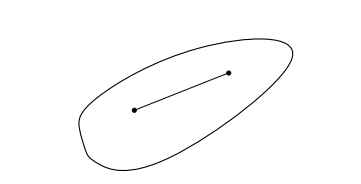
\includegraphics[width=0.8\textwidth]{figure/ch1/convex_set1.png}
        \caption{an example of a convex set}
    \end{minipage}%
    \begin{minipage}[t]{0.5\linewidth}
        \centering
        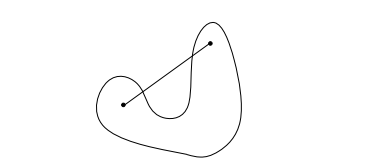
\includegraphics[width=0.8\textwidth]{figure/ch1/non_convex_set1.png}
        \caption{an example of a non convex set}
    \end{minipage}
\end{figure}


\begin{definition}{
    (Convex Function) % 定理的名字
  }{Convex Function
  }
    {
        a function $f: \Omega \rightarrow \R$ is convex, if $\Omega$ is convex and if
         \begin{equation}
            \forall x,y \in \Omega, t\in [0,1]: f(x+t(y-x))\leq f(x)+t(f(y)-f(x)). 
         \end{equation}
    }
\end{definition}
\begin{remark}
    $f(x+t(y-x))\leq f(x)+t(f(y)-f(x)) \Longleftrightarrow 
    f(ty+(1-t)x) \leq tf(y) + (1-t)f(x) $. As $x,y$ are arbitrary points, we can say $f$ is convex function if
    \ $\forall x,y \in \Omega, t\in [0,1]: f(tx+(1-t)y)\leq tf(x)+(1-t)f(y)$. 
\end{remark}
\begin{remark}
    This definition is equivalent to saying that
    all secants are above graph.
\end{remark}


\begin{figure}[htbp]
    \centering
    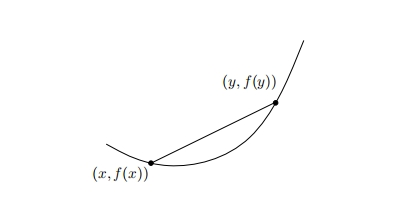
\includegraphics[width=0.6\textwidth]{figure/ch1/secant_above_graph1.png}
    \caption{For a convex function, the line segment \\ between any two points on the graph lies
    above the graph}
\end{figure}

\begin{definition}{
    (Convex Optimizaiton Problem) % 定理的名字
  }{% label
  }
    {
        an optimization problem with 
        \begin{itemize}
            \item a convex feasible set $\Omega$ and 
            \item a convex objective function $f: \Omega\rightarrow\R$
        
        \end{itemize}
        is called a "convex Optimization problem"
    }
\end{definition}






\begin{theorem}{
    (Local Implies Global Optimality for Convex Problems)
}{}
    {
        for a convex Optimization problem, every local minimum is also a global one. 
    }
\end{theorem}





\begin{proofsolution}
   
    \textcolor{LightRed}{
        Consider a local minimum $x^*$ of the convex optimization problem
        \begin{equation}
            \begin{split}
                \min_{x\in \R^n} f(x)\\
                s.t. x\in \Omega \nonumber
            \end{split}
        \end{equation}
        We will show that for each y $\in \Omega$ it holds $f(y)\geq f(x^*)$. 
    }

    Suppose that $x^*$ is not the global minmium, that is $\exists \ \widetilde{x} \in \Omega \ s.t. \ f(\widetilde{x})<f(x^*)$. \par
    Consider the line segement $x(t)=tx^*+(1-t)\widetilde{x}, t\in [0,1]$, 
        noting that $x(t)\in \Omega$ by the convexity of $\Omega$. 
        By the convexity of $f$,
        \begin{equation*}
            f(x(t))\leq tf(x^*)+(1-t)f(\widetilde{x})<tf(x^*)+(1-t)f(x^*)=f(x^*),\forall t\in [0,1]
        \end{equation*}
    \par
    As $x^*$ is a local minmium, we know that $\exists N$($N$ is a neighbourhood of $x^*$), $\forall x\in N$, $f(x)\geq f(x^*)$. 
        We can pick $t$ sufficiently to $1$ such that $x(t) \in N$. Then $f(x(t)) \geq  f(x^*)$. 
        This is a contradiction as $f(x(t)) < f(x^*)$ by the above inequality.
    \par
    Hence, $x^*$ is the global minimum. 
\end{proofsolution}

%%%%%%%%%ch1 section1 end%%%%%%%%

%%%%%%%%%ch2 section2%%%%%%%%%%%%

\section{How to Check Convexity of Functions?}

\begin{theorem}{
    (Convexity for $C^1$ Functions)
}{}
    {
        Assume that $f:\Omega\rightarrow\R$ is continuously differentiable
        and $\Omega$ is convex. Then it holds that $f$ is convex if and only if 
        \begin{equation}\label{eq:one_order_convexity_check}
            \forall x,y \in \Omega : f(y)\geq f(x) + (\nabla f(x))^T(y-x)
        \end{equation}
        $i.e.$ tangents lie below the graph. \\
    }
\end{theorem}

\begin{remark}
    The gradient (or gradient vector field) of a scalar function $f(x_1, x_2, x_3, …, x_n)$ is denoted $\nabla f$ and
    is a row vector. 
\end{remark}

\begin{figure}[htbp]
    \centering
    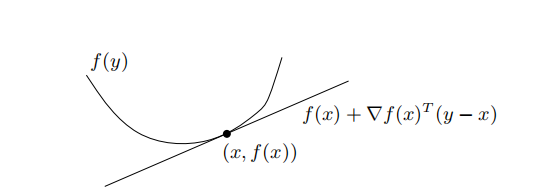
\includegraphics[width=0.6\textwidth]{figure/ch1/check_convexity1.png}
    \caption{}
\end{figure}

\begin{proofsolution}
    "$\Rightarrow$": If $f$ is convex, by definition, $\forall x\in (0,1]$, 
    \begin{equation*}
        \begin{split}
        f(x+t(y-x))\leq f(x)+t(f(y)-f(x)) \\
        \Longrightarrow f(y)-f(x)\geq \frac{f(x+t(y-x))-f(x)}{t(y-x)}\cdot (y-x)
        \end{split}
    \end{equation*}
    As $t\rightarrow 0$, we get 
    \begin{equation*}
        f(y)-f(x)\geq (\nabla f(x))^T \cdot (y-x). 
    \end{equation*}
    "$\Leftarrow$": Take any $x,y\in \Omega$ , $t\in [0,1]$  and let
    \begin{equation*}
        z = tx+(1-t)y. 
    \end{equation*}
    As $\Omega$ is convex, we have $z \in \Omega$. Then, by \eqref{eq:one_order_convexity_check}
    \begin{align*}
        f(x) & \geq f(z) + (\nabla f(z))^T(x-z)\\
        f(y) & \geq f(z) + (\nabla f(z))^T(y-z). 
    \end{align*}
    Then, 
    \begin{align*}
        tf(x) + (1-t)f(y) &\geq tf(z) + t(\nabla f(z))^T(x-z) 
        + (1-t)(f(z) + (1-t)(\nabla f(z))^T(y-z))\\
        &= f(z) + (\nabla f(z))^T(tx+(1-t)y-z)\\
        &= f(z) + (\nabla f(z))^T(z-z)\\
        &= f(tx+(1-t)y). 
    \end{align*}
    By definition\ref{def:Convex Function}, $f$ is a convex function. 
\end{proofsolution}

\begin{definition}{(Generalized inequality for Symmetric Matrices)}{}
    {
        $B$ is a symmetric matrix in $\R^{n\times n}$. Define "$B\succcurlyeq 0$" if and only if $B$ is positive semi-definite. i.e.
        \begin{align*}
            B\succcurlyeq 0 &\Longleftrightarrow \forall z \in \R^n : z^TBz\geq 0\\
                       &\Longleftrightarrow \min\{eig(B)\}\geq 0 
        \end{align*}

    }
\end{definition}

\begin{remark}
    $B\succcurlyeq 0$$\Longleftrightarrow$ all eigenvalues of $B$ are non-negative real value. $B$ is a symmetric matrix $\Rightarrow$ all eigenvalues of $B$ is real value. 
\end{remark}

% \begin{theorem}{}{}
%     A function $f:\Omega\rightarrow \R$ is convex if and only if the function $g:\R\rightarrow \R$ given by
%     $g(t)=f(x+ty)$ is convex for all $x\in \Omega$ and all $y\in \R^n$. (The domain of $g$ here is all $t$ for which $x+ty$ is in $\Omega$). 
% \end{theorem}
% \begin{proofsolution}
%     Here's a simple solution. A function $f:\R^n\rightarrow\R$
%  is convex iff the set Γf={(x1,⋯,xn,y)|f(x1,⋯,xn)≤y}⊆Rn+1
%  is convex.

% Now consider the region above the graph of g(t)
% : ΓG={(t,c)|g(t)≤c}
% . But this set is just the intersection of Γf
%  with the plane centered at x
%  generated by the vectors (v,0)
%  and (0,1)
% . Since linear subspaces are convex, Γf
%  is convex, and the intersection of two convex bodies is still convex, Γg
%  is convex and so g
%  is convex.

% The reverse direction is similar. Suppose f
%  is not convex. Then Γf
%  is not convex, and there exist points a,b∈Γf
%  such that the line between a,b
%  is not entirely contained in Γf
% . Since by definition such a line cannot be vertical, it means that the projection of such a line on to the first n
%  coordinates is again a line, and so we may choose that as the line that g
%  picks out. But then g
%  is not convex for the same reason- the line between a
%  and b
%  is not wholly contained in Γg
% .
% \end{proofsolution}

\begin{theorem}{(Convexity for $C^2$ Functions)}{two_order_convexity_check}
    {
        Assume that $f: \Omega\rightarrow \R$ is twice continuously differentiable and $\Omega$ is convex and open. 
        Then it holds that $f$ is convex if and only if for all $x\in \Omega$ the Hessian is positive semi-definite, i.e.
        \begin{equation}\label{eq:two_order_convexity_check}
            \forall x\in \Omega : \nabla^2 f(x) \succcurlyeq 0. 
        \end{equation}
    }    
\end{theorem}

\begin{proofsolution}
    Using Taylor expansion.
\end{proofsolution}


\begin{theorem}{}{}
    Consider an unconstrained optimization problem
    \begin{align*}
        \min f(x)\\
        s.t.\  x\in \R^n,
    \end{align*}
    where $f:\R^n\rightarrow \R$ is convex and differentiable. Then, 
    \begin{align*}
        \nabla f(x^*)=0 \Longleftrightarrow f(x)\geq f(x^*), \forall x\in dom(f). 
    \end{align*}
\end{theorem}

\begin{proofsolution}

\end{proofsolution}


\begin{theorem}{}{}
    Consider an optimization problem
    \begin{align*}
        \min f(x)\\
        s.t.\  x\in \Omega,
    \end{align*}
    where $f:\R^n\rightarrow \R$ is convex and differentiable and $\Omega$ is convex. Then for any $x^*\in \Omega$, 
    \begin{align*}
        \nabla f(x^*)(y-x^*)\geq 0, \forall y\in \Omega \Longleftrightarrow f(x)\geq f(x^*), \forall x\in \Omega.  
    \end{align*}
\end{theorem}

\begin{proofsolution}

\end{proofsolution}


%%%%%%%%

%%%%%%%%



\chapter{Descent Algorithms}\label{chp:descent algorithms}

\section{Motivation}

Let's recall our unconstrained optimization problem:
\begin{equation*}
    \min_{x} f(x), 
\end{equation*}
where $f:\R^n\rightarrow \R$.

\par
\noindent \textbf{Where we stand so far:}
\begin{itemize}
    \item Learned about some structural properties of local optimal solutions (first
    and second order conditions for optimality).
    \item Learned that for convex problems, local optima are automatically global.
\end{itemize}
\par 
But how to find a local optimum?
How to even find a stationary point (i.e., a point where the gradient
vanishes)? Recall that this would suffice for global optimality if is
convex.
We now begin to see some algorithms for this purpose. 
These will be iterative algorithms: start at a point, jump to a new point
that hopefully has a lower objective value and continue. 


\section{Descent Algorithms Overview}
\subsection{Iterative Form}
\noindent \textbf{General form of the iterations:}
\begin{equation*}
    x_{k+1} = x_k+\alpha_k d_k
\end{equation*}
\noindent where,
\begin{itemize}
    \item $k\in \Z_+$ : iteration number
    \item $x_k\in \R^n$ : current point
    \item $d_k\in R^n$ : direction to move along at iteration $k$
    \item $x_{k+1} \in \R^n$: next point
    \item $\alpha_k \in \R_+$: step size at iteration $k$.
\end{itemize}
\noindent Goal is to make the sequence $\{f(x_k)\}$
decrease as much as possible. But how to choose $d_k$? How to choose $\alpha_k$?
In first order method, the direction to move along at step is chosen
"based on information from" $\nabla f(x)$". Why is $\nabla f(x)$ a natural vector to look at? Lemmas \ref{lem:maximum rate of decrease} and \ref{lem:descent direction} below provide two reasons.

\begin{lemma}{}{maximum rate of decrease}
    $f\in C^1$. Consider yourself sitting at a point $x\in \R^n$ and looking (locally) at
    the value of the function $f$ in all directions around you. The direction with the
    maximum rate of decrease is along $-\nabla f(x)$. 
\end{lemma}


\begin{remark}
    When we speak of direction, the magnitude of the vector does not
matter; e.g., $\nabla f(X), 5\nabla f(x), \frac{\nabla f(x)}{20}$
 all are in the same direction.
\end{remark}

\begin{proofsolution}
    Consider a point $x$, a direction $d$, and the univariate function
    \begin{equation*}
        g(\alpha) = f(x+\alpha \frac{d}{||d||}). 
    \end{equation*}
    As the rate of change of $f$ at $x$ in direction $d$(derivative in direction $d$) is
    \begin{align*}
        \nabla_d f(x) &= \lim_{\alpha \rightarrow 0}\frac{f(x+\alpha \frac{d}{||d||}) - f(x)}{\alpha}=\lim_{\alpha\rightarrow 0}\frac{g(\alpha)-g(0)}{\alpha}=g'(0)\\
                &=(\nabla f(x))^T\frac{d}{||d||}=\frac{1}{||d||}<\nabla f(x),d>, 
    \end{align*}
    by the Cauchy-Schwarz inequality, we have:
    \begin{align*}
        -\frac{d}{||d||}\cdot ||\nabla f(x)|| \cdot ||d||\leq \frac{1}{||d||}<\nabla f(x),d>\leq \frac{d}{||d||}\cdot ||\nabla f(x)|| \cdot ||d||, 
    \end{align*}
    which after simplifying gives
    \begin{align*}
        -||\nabla f(x)|| \leq \frac{1}{||d||}<\nabla f(x),d>\leq||\nabla f(x)|| .  
    \end{align*}
    So $\nabla_d f(x)$ cannot be larger than $||f(x)||$, or smaller than $-||f(x)||$. However, if we take $d=\nabla f(x)$, the right inequality is achieved:
    \begin{align*}
        \frac{1}{||\nabla f(x)||}<\nabla f(x),\nabla f(x)>=\frac{1}{||\nabla f(x)||}\cdot ||\nabla f(x)||^2=||\nabla f(x)||. 
    \end{align*}
    Similarly, if we take $d=-\nabla f(x)$, then the left inequality is achieved. 
\end{proofsolution}


\begin{definition}{}{descent direction}
    For a given point $x\in R^n$, a direction $d\in \R^n$ is called a desent direction, if there exists $\bar{\alpha}>0$ such that
    \begin{align*}
        f(x+\alpha d)<f(x),\forall \alpha\in (0,\bar{\alpha})
    \end{align*}
\end{definition}

\begin{lemma}{}{descent direction}
    {
        Consider a point $x\in \R^n$. Any direction $d$ satisfying
        \begin{align*}
            \inner{\nabla f(x)}{d}<0
        \end{align*}
        is a descent direction.(In particular, $- \nabla f(x)$ is a desent direction.)
    }
\end{lemma}

\begin{remark}
    The condition $<\nabla f(x),d><0$ in Lemma \ref{lem:descent direction} geometrically means that
the vectors and make an angle of more than 90 degrees (on the plane
that contains them). \\
Why?(Hint: $<\nabla f(x),d>=||\nabla f(x)||\cdot ||d||\cdot cos\theta$)
\end{remark}

\begin{proofsolution}
    By Taylor's theorem, we have
    \begin{align*}
        f(x+\alpha d) = f(x) + \alpha \nabla f(x)^T d + o(\alpha).
    \end{align*}
    Since $\lim_{\alpha\rightarrow 0} \frac{|o(\alpha)|}{\alpha}=0$, there exists $\bar{\alpha}>0$ such that
    \begin{align*}
        \frac{|o(\alpha)|}{\alpha}<|\nabla f(x)^Td|,\forall \alpha\in(0,\bar{\alpha}).
    \end{align*}
    This, together with our assumption that $\nabla f(x)^Td<0$, implies that $\forall \alpha\in (0,\bar{\alpha})$ we must have:
    \begin{align*}
        f(x+\alpha d)&<f(x)+\alpha \nabla f(x)^T d + \alpha |\nabla f(x)^Td|\\
                    &<f(x)+\alpha \nabla f(x)^T d - \alpha \nabla f(x)^Td\\
                    &<f(x)
    \end{align*}
    Hence, by Definition \ref{def:descent direction} , $d$ is a descent direction.
\end{proofsolution}

\begin{lemma}{}{descent direction with pdmatrix}
    Consider any positive definite matrix $B$. For any point $x$, 
 with $\nabla f(x)\neq 0$, the direction $-B\nabla f(x)$ is a descent direction. 
\end{lemma}
\begin{proofsolution}
    By the assumption that $B$ is positive define, we have 
    \begin{align*}
        \inner{\nabla f(x)}{-B\nabla f(x)}=-\nabla f(x)^TB\nabla f(x)<0.
    \end{align*}
\end{proofsolution}

Lemma \ref{lem:descent direction with pdmatrix} suggets a general paradigm for our descent algorithms:
\begin{align*}
    x_{k+1} = x_k - \alpha_k B_k \nabla f(x_k), (\text{with}\ B_k\succ 0, \forall k).
\end{align*}

\noindent \textbf{Common choices of descent direction:}
\begin{itemize}
    \item Steepest Descent: $B_k=I,\forall k$.
    \item[] Simplest descent direction but not always the fastest.
    \item  Newton Direction: $B_k=(\nabla^2 f(x_k))^{-1}$, assuming $\nabla^2 f(x)\succ 0, \forall k$.
    \item[]  More expensive, but can have much faster convergence.
    \item Modified Newton Direction: $B_k=(\nabla^2f(x_0))^{-1},\forall k$
    \item[] Compute Newton direction only at the beginning, or once every M steps.
\end{itemize}

\noindent \textbf{Common choices of the step size $\alpha_k$: }
\begin{itemize}
    \item Constant step size: $\alpha_k=s,\forall k(s>0)$
        \begin{itemize}
            \item[*] Simplest rule to implement, but may not converge if $s$ too large; may
            be too slow if $s$ too small.
        \end{itemize}
    \item Diminishing step size: $\alpha_k\rightarrow 0$, $\sum\limits_{k=1}^{\infty}\alpha_k = \infty$. (e.g., $\alpha_k=\frac{1}{k}$)
    \item Minimization rule (exact line search): $\alpha_k = argmin_{\alpha\geq 0} f(x_k+\alpha_k d_k)$
        \begin{itemize}
            \item[*] A minimization problem itself, but an easier one (one dimensional).
            \item[*] If $f$ convex, the one dimensional minimization problem also convex  
        \end{itemize}
    \item Successive step size reduction: well-known examples are Armijo rule
    and Wolf rule. We will cover Armijo
    in the following chapter.
        \begin{itemize}
            \item[*] Try to ensure enough decrease in line search without spending time
            to solve $\alpha_k$ to optimality.
        \end{itemize}
\end{itemize}

\subsection{Stopping Criteria}
Once we have a rule for choosing the search direction and the step size,
we are good to go for running the algorithm. Typically the initial point $x_0$ is picked randomly, or if we have a guess for
the location of local minima, we pick $x_0$ close to them. But when to stop the algorithm? Some common choices ( $\epsilon>0$ is a small prescribed threshold):
\begin{itemize}
    \item $||\nabla f(x)||<\epsilon$
    \item[]  {If we have $\nabla f(x_k)=0$, our iterates stop moving. 
    We have found a point satisfying the first order necessary condition for optimality. 
    This is what we are aiming for. }
    \item $|f(x_{k+1})-f(x_k)|<\epsilon$
    \item[]  Improvements in function value are saturating.
    \item $||x_{k+1}-x_k||<\epsilon$
    \item[] Movement between iterates has become small.
\end{itemize}





\section{Rates of Convergence}
Now we make precise a useful notion of speed or rate of convergence, which is convenient for our convergence analysis.

\begin{definition}{}{}
    {
    Let $\{x_k\}$ converge to $x^*$. We say the convergence is of order $p$($\geq 1$) and with factor $\gamma$($>0$), if $\exists k_0$ such that $\forall k\geq k_0$, 
    \begin{align*}
        ||x_{k+1}-x^*|| \leq \gamma || x_k -x^*||^p.
    \end{align*}
    }
\end{definition}
Make sure the following comments make sense:









\section{Reference}
\begin{itemize}
    \item \href{https://www.princeton.edu/~aaa/Public/Teaching/ORF363_COS323/F14/ORF363_COS323_F14_Lec8.pdf}{lecture notes from princeton university}
\end{itemize}
\chapter{Gradient Descent}\label{chp:gradient descent}


\section{Convergence}
\begin{proposition}
    Suppose $f$ is convex and in $C^1$. The following statements are equivalent.\\
    (1) Lipschitz continuity of $\nabla f(x)$: there exists an $L>0$ such that
    \begin{align*}
        ||\nabla f(x)-\nabla f(y)||\leqs L||x-y||
    \end{align*}
\end{proposition}


\begin{theorem}{}{}
    Assume that $f : \R^n \rightarrow \R$ is convex and differentiable, and additionally
    \begin{align*}
        ||\nabla f(x)-\nabla f(y)||\leq L||x-y||,\forall x,y
    \end{align*}
    i.e. $\nabla f$ is Lipschitz continuous with constant $L>0$. Then Gradient Descent with $0\leq \alpha_k\leq \frac{1}{L}$ satisfies
    \begin{align*}
        f(x_k)-f(x^*)\leq \frac{||x_0-x^*||^2}{2\alpha_k k}.
    \end{align*}
    i.e. 
\end{theorem}

\begin{proofsolution}
    1
\end{proofsolution}



\begin{remark}
    proof reference: \href{https://www.cs.cmu.edu/~ggordon/10725-F12/scribes/10725_Lecture5.pdf}{notes from cmu}
\end{remark}

todo: add theorem when f is strongly convex

\section{Exact Line Search}

\section{Barzilai-Borwein (BB) method}


In the next chapter, we will introduce more about line search to choose appropriate step size. 

\section{Reference}
\begin{itemize}
    \item Convergence analysis: \href{https://www.math.cuhk.edu.hk/course_builder/1617/math6211a/cvxop.pdf}{lecture notes from cuhk}
    \item Exact Line Search: \href{https://www.princeton.edu/~aaa/Public/Teaching/ORF363_COS323/F23/ORF363_COS323_F23_Lec8.pdf}{lecture notes from princeton university}
    \item BB Method: \href{https://www.cmor-faculty.rice.edu/~yzhang/caam565/L1_reg/BB-step.pdf}{lecture notes from UCLA}
\end{itemize}
\chapter{Line Search}\label{chp:Line Search}


\section{Motivation}
    In last chapter, we have introduce the iterative form for an unconstrained optimization problem
    \begin{align*}
        \min_{x} f(x),
    \end{align*}
    where $f:\R^n\rightarrow \R$. Suppose that $x_k$ is our current best estimate of a solution to the problem. 
    A standard method for improving the estimate $x_k$ is to choose a direction of search $d \in \R^n$ and then compute a step length $\alpha \in \R^n$ so that $x_k+\alpha d$ approximately optimizes f. 
    The new estimate for the solution to the problem is then $x_{k+1}=x_k + \alpha d$. The procedure for choosing $\alpha$ is called a line search method. If $\alpha$ is taken to be the
    global solution to the following problem
    \begin{align*}
        min_{\alpha \in \R} f(x_k+\alpha d), 
    \end{align*}
    then $\alpha$ is called the Curry step length.  However, except in certain very special cases, the
    Curry step length is far too costly to compute. For this reason we focus on a few easily
    computed step lengths. We begin the simplest and the most commonly used line search
    method called backtracking.     
    
\section{The Basic Backtracking Algorithm}
In the backtracking line search we assume
that $f:\R^n\rightarrow \R$ is is differentiable and that we are given a direction $d$ of strict desent at the current point $x_k$, that is $f'(x_k;d)=<\nabla f(x_k),d><0$.

\begin{algorithm}[H]
    \SetKwInOut{Input}{input}
    \SetKwInOut{Output}{output}
    \Input{$\gamma \in (0,1)$ , $c_1\in (0,1)$, desent direction $d$, inital step size $\hat{\alpha}$ and current solution $x_k$}
    \Output{the next solution $x_{k+1}$}
    \BlankLine
    $\alpha=\hat{\alpha}$\\
    \While{ $f(x_k+\alpha d)>f(x_k) + c_1\alpha f'(x_k;d)$} {
        $a\leftarrow \gamma\alpha$\;
    }
    $\alpha^*=\alpha$\\
    \Return $x_{k+1}=x_k+\alpha^* d$
    \caption{Descent Algorithm with Backtracking Line Search at iteration $k$}
    \label{alg:bls}
\end{algorithm}
The backtracking line search method forms the basic structure upon which most line search
methods are built. Due to the importance of this method, we take a moment to emphasize
its key features.
\par
(i) The search direction $d$ must satisfy
\begin{equation*}
    f'(x_k;d)<0. 
\end{equation*}
Any direction satisfying this strict inequality is called a direction of strict descent for
$f$ at $x_k$.
\par 
(ii) In algorithm, we require that the step length $\alpha^*$ be chosen so that
\begin{equation*}
    f(x_k+\alpha^* d)\leq f(x_k) + c_1\alpha^* f'(x_k;d)
\end{equation*}
This inequality is called the Armijo-Goldstein inequality. It is named after the two
researchers to first use it in the design of line search routines (Allen Goldstein is a Professor Emeritus here at the University of Washington). 
Since $f'(x_k;d)<0$, this inequality
guarantees that
    \begin{equation*}
        f(x_k+\alpha^* d)< f(x_k). 
    \end{equation*}
And by definition \ref{def:descent direction}, if $d$ is a direction of strict descent, 
it is always possible to choose $\alpha^*$ so that $f(x_k+\alpha^* d)< f(x_k)$.  
But the Armijo-Goldstein inequality is a somewhat stronger statement. We claim that there exists $\alpha$ satisfying the inequality as $f'(x_k;d)<0$, 
\begin{equation*}
    \lim_{\alpha\rightarrow 0^+} \frac{f(x_k+\alpha d)-f(x_k)}{\alpha} = f'(x_k;d)<c_1f'(x_k;d)<0. 
\end{equation*}
Hence, there is a $\bar{\alpha}>0$ such that 
\begin{equation*}
    \frac{f(x_k+\alpha d)-f(x_k)}{\alpha} \leq c_1f'(x_k;d), \forall t\in (0,\bar{t}),
\end{equation*}
that is 
\begin{equation*}
    f(x_k+\alpha d)\leq f(x_k) + c_1\alpha f'(x_k;d),\forall \alpha \in (0,\bar{\alpha}).
\end{equation*}
\par
(iii) The Armijo-Goldstein inequality is known as a condition of sufficient decrease. It is
essential that we do not choose $\alpha^*$ too small. Because $\alpha^*=\gamma^j \hat{\alpha}$, where $j=\min\{j=0,1,2,...|f(x_k+\gamma^j \hat{\alpha} d)\leq f(x_k) + c_1\gamma^j \hat{\alpha} f'(x_k;d)\}$. 
In general, we always wish to choose $\alpha^*$ as large as possible since it is often the factor that some effort was put into the selection of the
search direction $d$. Indeed, as we will see, for Newton's method we must take $\alpha^*=1$ in order to achieve rapid local convergence.
\par
(iv) There is a balance that must be struck between taking $\alpha^*$ as large as possible and not
having to evaluating the function at many points. Such a balance is obtained with
an appropriate selection of the parameters $\gamma$ and $c_1$. Typically one takes $\gamma \in [0.5, 0.8]$
while $c_1 \in [0.001, 0.1]$ with adjustments depending on the cost of function evaluation
and degree of nonlinearity.

\section{Convergence for Backtracking Line Search}

\section{The Wolfe Conditions}
In exact line search method, we want to gain the stepsize $\aleph_k$ satisfying 
\begin{equation*}
    f(x_k+\alpha_k d_k) = \min_{\alpha\in \R}f(x_k+\alpha d_k).
\end{equation*} 
Let $g(\alpha)=f(x_k+\alpha d_k)$, the first-order optimality conditions tell us that we should find $\alpha$ satisfying $0=g'(\alpha)=\nabla f(x_k+\alpha d_k)^Td_k$. The
Wolfe conditions try to combine the Armijo-Goldstein sufficient decrease condition with a
condition that tries to push $0=\nabla f(x_k+\alpha d_k)^Td_k$ either toward zero, or at least to a point
where the search direction $c_k$ is less of a direction of descent. To describe these line search
conditions, we take parameters $0<c_1<c_2<1$. 
\par
\noindent \textbf{Weak Wolfe Conditions}
\begin{subequations}
    \begin{align}
        f(x_k+\alpha_k d_k) &\leq f(x_k)+c_1\alpha_kf'(x_k;d_k)\label{eq:Weak Wolfe Conditions a}\\
        c_2f'(x_k;d_k)&\leq f'(x_k+\alpha_kd_k;d_k).\label{eq:Weak Wolfe Conditions b}
    \end{align}
    \end{subequations}


\par
\noindent\textbf{Strong Wolfe Conditions}
\begin{subequations}
    \begin{align}
        f(x_k+\alpha_k d_k) &\leq f(x_k)+c_1\alpha_kf'(x_k;d_k)\label{eq:Strong Wolfe Conditions a}\\
        |f'(x_k+\alpha_kd_k;d_k)| &\leq c_2|f'(x_k;d_k)| .\label{eq:Strong Wolfe Conditions b}
    \end{align}
\end{subequations}
The weak Wolfe condition (\ref{eq:Weak Wolfe Conditions b}) tries to make $d_k$
less of a direction of descent (and possibly a direction of ascent) at the new point, 
while the strong Wolfe condition (\ref{eq:Strong Wolfe Conditions b}) tries to push the
directional derivative in the direction $d_k$
closer to zero at the new point. Imposing one or
the other of the Wolfe conditions on a line search procedure has become standard practice
for optimization software based on line search methods.
\par
We now give a result showing that there exists stepsizes satisfying the weak Wolfe conditions. 
A similar result (with a similar proof) holds for the strong Wolfe conditions.       

\begin{lemma}{}{}
    Let $f:\R^n\rightarrow \R$ be continuously differentiable and suppose that $x,d\in \R^n$ are such
    that the set $\{f(x+\alpha d)|\alpha \geq 0\}$ is bounded below and $f'(x;d)<0$, then for each $0<c_1<c_2<1$ the set
    \begin{align*}
       S= \{\alpha |\alpha >0, f'(x+\alpha d;d)\geq c_2f'(x;d) \ and\  f(x+\alpha d)\leq f(x)+c_1\alpha f'(x;d)\}
    \end{align*}
    has non-empty interior.
\end{lemma}
\begin{proofsolution}
    Let $\phi(\alpha) = f(x+\alpha d)-(f(x)+c_1\alpha f'(x;d))$. Then 
    \begin{align*}
        \phi(0)&=0 \\
        \phi'(0)&=(1-c_1)f'(x;d)<0.
    \end{align*}
    So there exists $\bar{\alpha}>0$
    such that $\phi(\alpha)<0$ for $\alpha \in (0,\bar{\alpha})$. Moreover, since $f'(x;d)<0$ and $\{f(x+\alpha d)|\alpha>0\}$ is bounded below, 
    we have $\phi(\alpha)\rightarrow +\infty$ as $\alpha\rightarrow +\infty$. Hence, by the continuity of $f$, there exies $\hat{\alpha}>0$ such that $\phi(\hat{\alpha})=0$. Let $\alpha_0= \inf{\alpha|\alpha\geq 0,\phi(\alpha)=0}$.
    \par
    Since $\phi(0)=\phi(\alpha_0)$ and $\phi(\alpha)$ is continuously differentiable, by Rolle's theorem, there must exists $\widetilde{\alpha}\in (0,\alpha_0)$ with $\phi'(\widetilde{\alpha})=0$. That is, 
    \begin{align*}
        & \nabla f(x+\widetilde{\alpha}d)^Td-c_1\nabla f(x)^Td=0\\
      \Rightarrow  &\nabla f(x+\widetilde{\alpha}d)^Td = c_1\nabla f(x)^Td > c_2\nabla f(x)^Td.
    \end{align*}
    From the definition of $\alpha_0$ and the fact that $\widetilde{\alpha}\in (0,\alpha_0)$, we also have
    \begin{align*}
        f(x+\widetilde{\alpha} d)-(f(x)+c_1\widetilde{\alpha} f'(x;d))<0.
    \end{align*}
    Hence, $\widetilde{\alpha}\in \inf(S)$ and $\inf(S)\neq \emptyset$.
\end{proofsolution}

\section{A Bisection Method for the Weak Wolfe Conditions}

\section{Convergence for Line Search Based on the Weak Wolfe Conditions}


\section{Interpolation Line Search}

\section{Reference}

\begin{itemize}
    \item Armijo \& Wolfe conditions: \href{https://sites.math.washington.edu/~burke/crs/408/notes/nlp/line.pdf}{lecture note from washington university}
    \item interpolation line search: 
    \begin{itemize} 
        \item[*] \href{http://www.ece.northwestern.edu/local-apps/matlabhelp/toolbox/optim/tutori5b.html}{matlab optimizaiton toolbox tutorial}
        \item[*] \href{https://www-personal.umich.edu/~murty/611/611slides9.pdf}{lecture notes from michigan university}
    \end{itemize}
\end{itemize}
\chapter{Newton's Method}\label{chp:Newton Method}

\section{Motivation}




In this chapter we study the choice of search directions used in our basic updating scheme
\begin{align*}
    x_{k+1} = x_k +\alpha_k d_k. 
\end{align*}
for solving
\begin{align*}
    \mathcal{P}:\min_{x\in\R^n} f(x).
\end{align*}
In the previous lecture, we saw the general framework of descent
algorithms, with several choices for the step size and the descent
direction. Today, we see a wonderful descent method with superlinear (in fact
quadratic) rate of convergence: the Newton algorithm.
\par 
The Newton's method is nothing but a descent method with a specific
choice of a descent direction; one that iteratively adjusts itself to the local
geometry of the function to be minimized.
\par
In practice, Newton's method can converge with much fewer iterations
than gradient methods. For example, for quadratic functions, while we
saw that gradient methods can zigzag for a long time (depending on the
underlying condition number), Newton's method will always get the
optimal solution in a single step. The cost that we pay for fast convergence is the need to 
\par
(1) access second order information (i.e., derivatives of first and second order), and 
\par
(2) solve a linear system of equations at every step of the algorithm.

\section{Pure Newton method }
Recall the general form of our descent methods:
\begin{align*}
    x_{k+1}=x_k+\alpha_kd_k.
\end{align*}
Let us have $\alpha_k=1,\forall k$ for now.  So we take full steps at
each iteration. (This is sometimes called the pure
Newton method.) Newton's method is simply the following choice for the
descent direction:
\begin{align*}
    d_k = -(\nabla^2 f(x))^{-1}\nabla f(x_k).
\end{align*}
And iteration only well-defined when $\nabla^2 f(x)$ is invertible.
\par 
But Where does $d_k$ come from? One motivation is minimizing a quadratic approximation of the function
sequentially. 
\par
Around the current iterate $x_k$, $f(x)$ can be approximated by:
\begin{align*}
    f(x)\approx q(x):= f(x_k)+\nabla f(x_k)^T(x-x_k)+\frac{1}{2}(x-x_k)^T\nabla^2f(x_k)(x-x_k),
\end{align*}
which is the quadratic Taylor expansion of $f(x)$ at $x = x_k$. Notice that $q(x)$ is a quadratic function, which is minimized by solving
$\nabla q(x) = 0$. Since the gradient of $q(x)$ is:
\begin{align*}
    \nabla q(x) = \nabla f(x_k) + \nabla^2 f(x_k)(x-x_k), 
\end{align*}
we therefore are motivated to solve:
\begin{align*}
    \nabla f(x_k) + \nabla^2 f(x_k)(x-x_k) = 0,
\end{align*}
which yields
\begin{align*}
    x-x_k = -(\nabla^2 f(x))^{-1}\nabla f(x_k). 
\end{align*}
This leads to the pure Newton method for solving $\mathcal{P}$.


\textcolor{red}{add: solve least square using pure newton method}

\section{Quadratic Convergence of Newton's Method}

\begin{proposition}{}{}
    If $\nabla^2 f(x)\succ 0$ and $d=-(\nabla^2 f(x))^{-1}f(x)\neq 0$, then $d$ is a desent direction. 
\end{proposition}
\begin{proof}
    It is sufficient to show that $\nabla f(x)^T d=-\nabla f(x)^T\nabla^2 f(x)^{-1}\nabla f(x)<0$. 
    This will clearly be the case if $(\nabla^2 f(x))^{-1}\succ 0$. Since $\nabla^2 f(x)\succ 0$, if $y\neq 0$,
    \begin{align*}
        0<(\nabla^2 f(x)^{-1} y)^T\nabla^2f(x)(\nabla^2 f(x)^{-1}y) = y^T\nabla^2 f(x)^{-1}y,
    \end{align*}
    thereby showing that $\nabla^2f(x)^{-1}\succ0$.
\end{proof}

\begin{proposition}{}{}
    Suppose that $f(x)$ is twice differentiable. Then
    \begin{align*}
        \nabla f(z) - \nabla f(x) = \int_{0}^{1} \nabla^2f(x+t(z-x))(z-x) dt.
    \end{align*}
\end{proposition}
\begin{proof}
    Let $\phi(t)=\nabla f(x+t(z-x))$. Then $\phi(0)=\nabla f(x)$ and $\phi(1) = \nabla f(z)$, 
    and $\phi'(t)= \nabla^2 f(x+t(z-x)) (z-x)$. From Newton-Leibniz theorem, we have 
    \begin{align*}
        \nabla f(z) - \nabla f(x) &= \phi(1)-\phi(0)\\
                                  &= \int_{0}^{1} \phi'(t) dt\\
                                  &= \int_{0}^{1}\nabla^2 f(x+t(z-x))(z-x)dt.
    \end{align*}
\end{proof}


\begin{theorem}{}{}
    Suppose $f(x)$ is twice continuously differentiable and $x^*$ is a point for which $\nabla f(x^*)=0,\nabla^2 f(x^*)\succ 0$.
    Suppose that $\nabla^2 f(x)$ is Lipschitz continuous at a neighbourhood of $x^*$ (denoted by $\mathcal{N}_{\delta}(x^*)$), i.e.
    \begin{align*}
        ||\nabla^2 f(x)-\nabla^2 f(y)||\leq L||x-y||, \forall x,y \in \mathcal{N}_{\delta}(x^*).
    \end{align*}
    Then:\\
    (1) iterative sequence $\{x_k\}$ converges to $x^*$ if inital point is close to $x^*$(local convergence).\\
    (2) the convergence rate of (i) is  quadratic.\\
    (3) sequence $\{||\nabla f(x_k)||\}$ converges to $0$ and the convergence rate is quadratic.
\end{theorem}
\begin{proofsolution}
    Since $\nabla f(x^*)=0$, we have\\
    \textcolor{red}{$\nabla^2 f(x_k)^{-1}$ is pd since $x_k$ close to $x^*$ }
    \begin{align*}
        x_{k+1} - x^* &= x_k - \nabla^2 f(x_k)^{-1}\nabla f(x_k)-x^*\\
                      &= (x_k - x^*)-\nabla^2 f(x_k)^{-1}\nabla f(x_k)
                      &= \nabla^2 f(x_k)^{-1}(\nabla^2 f(x)(x_k-x^*)-(\nabla f(x_k)-\nabla f(x^*))).
    \end{align*}
\end{proofsolution}

In practice, to guarante the local convergence, we usually firstly use gradient descent to  

\section{Modified Newton Method}

There are some drawbacks of pure Newton method:
\par
(1) When $\nabla^2 f(x)$ is not positve-definite, Newton's direction may not be a descent direction.
\par
(2) When the inital point is far away from the optimal point, by choosing $\alpha_k=1$, we may not be able to obtain a convergent iterative sequence. 
This is because the Taylor approximation is limited in region.

\par 
Hence, something should be done to modified pure Newton's Method. 
In this section, we firstly introduce the modified Newton method with line search. 
The basic idea is: 
\par
(1) modified $\nabla^2 f(x)$ so that we can get a positve definite matrix. 
\par
(2) use line search method to choose step size.

\begin{algorithm}[H]
    \SetKwInOut{Input}{input}
    \SetKwInOut{Output}{output}
    \Input{current solution $x_k$}
    \Output{the next solution $x_{k+1}$}
    \BlankLine
    determined matrix $E_k$ such that $B_k\overset{def}{=} \nabla^2 f(x_k) + E_k$ is postive-definite and the condition number is small. \\
    solve the modified newton equation $B_kd_k=-\nabla f(x_k)$ to obtain desent direction $d_k$.\\
    use any line search condition to choose stepsize $\alpha_k$.\\
    \Return $x_{k+1}=x_k+\alpha_k d_k$
    \caption{modified Newton method with line search at iteration $k$}
    \label{alg:mnmls}
\end{algorithm}

\textcolor{red}{when the dimension is too big, the calculation of modified newton method is also expansive}

\section{Reference}
\begin{itemize}
    \item \href{https://www.princeton.edu/~aaa/Public/Teaching/ORF363_COS323/F23/ORF363_COS323_F23_Lec9.pdf}{lecture notes from princeton university}
    \item \href{https://ocw.mit.edu/courses/15-084j-nonlinear-programming-spring-2004/83159d56de04a7e7dc94d0348fa4ccda_lec3_newton_mthd.pdf}{lecture notes from MIT}
\end{itemize}
\chapter{Conjugate Direction Methods}\label{chp:Conjugate_direction}





\section{Reference}
\begin{itemize}
    \item \href{https://sites.math.washington.edu//~burke/crs/408/notes/nlp/cg.pdf}{lecture notes from washington university}
    \item \href{https://ocw.mit.edu/courses/15-084j-nonlinear-programming-spring-2004/resources/lec4_quad_form/}{lecture notes from mit}
\end{itemize}
\chapter{Quasi-Newton Methods}\label{chp:Quasi-Newton Methods}

\section{Motivation}


In last chapter, we have known that All of the search directions considered can be classified as Newton-like since they are all of
the form 
\begin{align*}
    d_k = -H_k\nabla f(x_k),
\end{align*}
where $H_k$ is a symmetric $n\times n$ matrix. If $H_k=\mu_k I$ for all $k$, the resulting search direction as a scaled steepest descent direction
with scale factors $mu_k$. More generally, we choose $H_k$ to approximate $\nabla^2 f(x_k)^{-1}$ in 
order to approximate Newton's method for optimization. The Newton method is important since it possesses rapid local convergence properties, and can be shown
to be scale independent. 

\section{Newton's Method for Solving Equations}
Newton's method is an iterative scheme
designed to solve nonlinear equations of the form
\begin{equation}
    g(x)=0,
    \label{eq:nonlinear equation}
\end{equation}
where $g:\R^n\rightarrow \R^n$ is assumed to be continuously differentiable. Many problems of importance can be posed in this way. In the context of the optimization problem $\mathcal{P}$, we wish 
to locate  critical points, that is, points at which $\nabla f(x)=0$. We begin our discussion of
Newton’s method in the usual context of equation solvng. 
\par 
Assume that the function $g$ in (\ref{eq:nonlinear equation}) is continuously differentiable and that we have an
approximate solution $x_0\in\R^n$. We now wish to improve on this approximation. If $x^*$ is a solution to (\ref{eq:nonlinear equation}), then
\begin{align*}
    0= g(x^*)=g(x_0)+g'(x_0)(x^*-x_0)+o(||x^*-x_0||).
\end{align*}
Thus, it is reasonable to suppose that the solution to the linearized
system
\begin{equation}
    0=g(x_0)+g'(x_0)(x-x_0)
    \label{eq:linearized system equation}
\end{equation}
is even closer. This is Newton’s method for finding the roots of the equation $g(x)=0$.  It
has one obvious pitfall. The solution $x=x_0- [g'(x_0)]^{-1}g(x_0)$ exists if and only if $g'(x_0)$ exists. 
\par 
For the sake of the present argument, we assume that $g'(x_0)^{-1}$ exists. Under this assumption, equation(\ref{eq:linearized system equation})  defines the iteration scheme,
\begin{equation}
    x_{k+1} = x_k - [g'(x_k)]^{-1}g(x_k), 
\end{equation}
called the Newton iteration. The associated direction
\begin{equation}
    d_k = - [g'(x_k)]^{-1}g(x_k).
\end{equation}
is called the Newton direction. We analyze the convergence behavior of this scheme under
the additional assumption that an approximation to $[g'(x_k)]^{-1}$ is available. We denote
this approximation by $H_k$. The resulting iteration scheme is 
\begin{equation}
    x_{k+1} = x_k -H_kg(x_k). 
\end{equation}
Methods of this type are called \textbf{Newton-Like methods}.
\section{Reference}
\begin{itemize}
    \item \href{https://sites.math.washington.edu/~burke/crs/408/notes/nlp/direction.pdf}{lecture notes from washington university}
    \item \href{https://math.ucsd.edu/sites/math.ucsd.edu/files/undergrad/honors-program/honors-theses/2019-2020/Jeb_Runnoe_Honors_Thesis.pdf}{lecture notes from ucsd}
    \item \href{https://www.stat.cmu.edu/~ryantibs/convexopt-F18/lectures/quasi-newton.pdf}{lecture notes from cornell}
    \item \href{https://www.cs.ccu.edu.tw/~wtchu/courses/2014s_OPT/Lectures/Chapter%2011%20Quasi-Newton%20Methods.pdf}{lecture notes from ccu}
\end{itemize}
\chapter{Trust Region}\label{chp:trust_region}

\section{Reference}
\begin{itemize}
    \item \href{https://acme.byu.edu/0000017a-1bb8-db63-a97e-7bfa0bd80000/vol2lab19trustregion-pdf}{lecture notes from brigham}
    \item \href{https://www.numerical.rl.ac.uk/people/nimg/course/lectures/raphael/lectures/lec6slides.4.pdf}{lecture notes from ox}
    \item \href{https://people.maths.ox.ac.uk/hauser/hauser_lecture3.pdf}{lecture notes from ox}
    \item \href{https://www.csie.ntu.edu.tw/~cjlin/papers/logistic.pdf}{Trust Region Newton Method for Large-Scale Logistic Regression}
\end{itemize}
\chapter{Nonlinear Least Squares Problem}\label{chp:nonlinear_least_Squares}

\section{Reference}
\begin{itemize}
    \item \href{https://people.duke.edu/~hpgavin/ExperimentalSystems/lm.pdf}{thesis from duke university}
    \item \href{https://www2.imm.dtu.dk/pubdb/edoc/imm3215.pdf}{lecutre nots from dtu}
    \item \href{https://vnav.mit.edu/material/17-18-NonLinearLeastSquares-notes.pdf}{lecture nots from vnav}
\end{itemize}

%%%%%%%%%%%%%%%%%%%%%%%%%%%%%%%%%%%%%%%part 2%%%%%%%%%%%%%%%%%%%%%%%%%% 
\part{Duality}

\part{Application}



% \part{}


%%%%%%%%%%%%%%%Content%%%%%%%%%%%%%%%
% % \mainmatter % separat the number of toc and mainmatter
% % !TEX root = ../notes_template.tex
\chapter*{Preface}


Notes mainly refer to the following resources:
Convex optimization & duality:
\begin{itemize}
    \item \href{https://web.stanford.edu/~boyd/cvxbook/}{Convex Optimizaiton. Stephen Boyd, Lieven Vandenberghe}
    \item \href{https://link.springer.com/book/10.1007/978-0-387-40065-5}{Numerical Optimization(2nd). Jorge Nocedal, Stephen J.Wright} 
    \item \href{https://cdn.syscop.de/publications/Diehl2016.pdf}{lecture notes from University of Freiburg}
    \item \href{https://faculty.ucmerced.edu/mcarreira-perpinan/teaching/EECS260/lecture-notes.pdf}{lecture notes from University of California}
    \item \href{https://www.uio.no/studier/emner/matnat/math/nedlagte-emner/MAT-INF2360/v13/matinf2360part3.pdf}{Lecture notes for the course MAT-INF2360}
    \item \href{https://www.numerical.rl.ac.uk/people/nimg/msc/lectures/paper.pdf}{An introduction to algorithms for nonlinear optimization} 
    \item \href{https://www.princeton.edu/~aaa/Public/Teaching/ORF523/S16/}{ORF 523 Convex and Conic Optimization}
    \item \href{}{lecture notes from School of Electrical Engineering at Korea Advanced Institute of Science and Technology}
    \item \href{https://www.stat.cmu.edu/~ryantibs/convexopt-F18/}{Convex Optimization: Fall 2018}
\end{itemize}


application:

\begin{itemize}
    \item \href{https://web.eecs.umich.edu/~fessler/course/598/}{Optimization methods for signal and image processing and machine learning}
\end{itemize}



% \par

all the codes in the notes are completed by python. You can get the codes in the following website:
\begin{itemize}
    \item -
\end{itemize}

\par
% In Part I, we will study the basic concepts and several
% mathematical definitions required to understand what convex optimization is as well as how to
% translate an interested problem into a convex problem. We will then explore five instances of
% convex optimization problems: LP, least-squares, QP, SOCP and SDP. Specifically we will focus
% on techniques which serve recognizing (and translating to) such problems. We will also study
% some prominent algorithms for solving such problems. 
% \par
% In Part II, we will study one of the key
% theories in the optimization field, called duality. There are two types of dualities: (1) strong
% duality; (2) weak duality. It turns out that the strong duality is quite useful for gaining some
% algorithmic insights for convex problems. 
% The weal duality helps dealing with difficult non-convex problems, by providing an approximated solution.
% \par 
% In part III, our focus is on continuous optimization (rather than discrete optimization) with special emphasis on nonlinear programming.
% We will Utilize the knowledge of PartI and PartII to mine the optimal solution conditions and 
% solving methods for nonlinear optimization problems. 







% \part{Mathematics}

% % !TEX root = ../notes_template.tex
\chapter{Discrete Math}\label{chp:discrete_math}


\section{Proof}

\begin{theorem}
\end{theorem}

\begin{solution}
By induction:
\end{solution}



\section{Quantifier}
\lipsum % dummy text - remove from real document

\section{Graph}
\citetitle{babaiGraphIsomorphismQuasipolynomial2016}
\cite{babaiGraphIsomorphismQuasipolynomial2016}

\section{Number theory}
Figure example
\begin{figure}[!ht]
    \centering
    \includegraphics[width=1\linewidth]{./figure/elliptic_curves.pdf}
    \caption{Elliptic curves \cite{childsUniversalComputationQuantum2009} }
\end{figure}


\section{Algorithm}
% \begin{center}
% \begin{minipage}{.9\linewidth}
% algorithm2e
% https://www.overleaf.com/learn/latex/Algorithms#The_algorithm2e_package
\begin{algorithm}[H]
    \SetKwInOut{Input}{input}
    \SetKwInOut{Output}{output}
    \Input{Integer $N$ and parameter $1^t$}
    \Output{A decision as to whether $N$ is prime or composite}
    \BlankLine
    \For{ $i = 1,2, \ldots, t$} {
        $a\leftarrow \qty{1,\dots,N_1}$\;
        \If{$a^{N-1} \neq 1 \mod{N}$}
    {\Return "composite"}
    }
    \Return "prime"
    \caption{Primality testing - first attempt}
    \label{alg:miller_rabin}
\end{algorithm}
% \end{minipage}
% \end{center}

% \part{Computer Science}
% % \input{./chapter/complexity.tex}
% % !TEX root = ../notes_template.tex
\chapter{Machine Learning}\label{chp:machine_learning}
\minitoc

\section{Regression}
% \gls{algorithm};
\subsection{Gradient descent}\label{sec:gradient_descent}
\gls{gd};
% \glsxtrshort{gd}

\section{Support Vector Machine}
\gls{svm};
% % \input{./chapter/algorithms.tex}

% \part{Physics}
% % !TEX root = ../notes_template.tex
\chapter{Quantum Mechanics}\label{chp:quantum_mechanics}
\minitoc

\section{Hamiltonian}
\gls{hamiltonian};
% \glsxtrshort{qm};

\section{Path Integral}
\gls{lagrangian}

\section{Quantum Field Theory}
\gls{qft};
% % \input{./chapter/quantum_field_theory.tex}

% % \begin{appendices}
% % % !TEX root = ../notes_template.tex
\chapter{Formulas}

\section{Gaussian distribution}\label{sec:gaussian_distribution}
\begin{Definition}[Gaussian distribution]\label{def:gaussian_distribution}
    \myindex{Gaussian distribution}
\end{Definition}

\begin{theorem}[Central limit theorem]\label{thm:central_limit_theorem}
\end{theorem}
% % \end{appendices}

% \backmatter

% %%%%%%%%%%%%%%% Reference %%%%%%%%%%%%%%%

% \printbibliography[heading=bibintoc]
% \printindex
\end{spacing}
\end{document}